\documentclass[journal]{IEEEtran}

% ---------------------------------------------------------------
% Packages
% ---------------------------------------------------------------
\usepackage[T1]{fontenc}
\usepackage[utf8]{inputenc}
\usepackage{amsmath,amssymb,amsfonts}
\usepackage{graphicx}
\usepackage{textcomp}
\usepackage{xcolor}
\usepackage{booktabs}
\usepackage{multirow}
\usepackage{url}
\usepackage{cite}
\usepackage{pgfplots}
\pgfplotsset{compat=1.18}
\usepackage{tikz}
\usetikzlibrary{shapes.geometric, arrows.meta, positioning, fit, backgrounds}
\usepackage{array}
\usepackage{siunitx}
\DeclareSIUnit{\dBm}{dBm}
\usepackage{dblfloatfix}

% ---------------------------------------------------------------
% TikZ block styles
% ---------------------------------------------------------------
\tikzset{
  blk/.style={
    rectangle, rounded corners=3pt, draw=black, fill=blue!9,
    text width=5.8em, align=center, minimum height=2.2em, font=\small
  },
  wblk/.style={
    rectangle, rounded corners=3pt, draw=black, fill=green!9,
    text width=8.2em, align=center, minimum height=2.2em, font=\small
  },
  oblk/.style={
    rectangle, rounded corners=3pt, draw=black, fill=orange!12,
    text width=6.5em, align=center, minimum height=2.2em, font=\small
  },
  rblk/.style={
    rectangle, rounded corners=3pt, draw=black, fill=red!8,
    text width=7.0em, align=center, minimum height=2.2em, font=\small
  },
  arr/.style={-Stealth, thick},
  stgbox/.style={
    rectangle, rounded corners=5pt,
    draw=black!55, dashed, thick, inner sep=7pt
  }
}

% ---------------------------------------------------------------
\begin{document}

\title{i-DECIDE: Proactive LTE Handover Prediction Using a Two-Stage\\
Deep Learning Pipeline on Real-World Drive-Test Data}

\author{Suraj~Meruva,~\IEEEmembership{Student Member,~IEEE}%
\thanks{S. Meruva is with the Department of Computer Science and
Engineering, Indian Institute of Information Technology Naya Raipur,
Chhattisgarh 493661, India (e-mail: meruva24102@iiitnr.edu.in).
Manuscript received 2026-06-17.}}

\markboth{IEEE Transactions on Vehicular Technology,~Vol.~XX,~No.~X,~2026}%
{Meruva: i-DECIDE Handover Prediction on Real-World Drive-Test Data}

\maketitle

% ---------------------------------------------------------------
\begin{abstract}
Proactive handover (HO) prediction in LTE networks is evaluated here
through a full, end-to-end deployment of the i-DECIDE two-stage deep
learning framework on a real-world vehicular drive-test log collected
from an operational Airtel LTE network in India. The measurement
campaign recorded 10\,301 LTE samples over four days from a single
User Equipment (UE) traversing an urban area, capturing 323 handover
events across 169 Physical Cell Identities (PCIs) at RSRP levels
ranging from $-129$ to $-60$~dBm. The first stage feeds 100-sample
RSRP windows into a stacked four-layer Long Short-Term Memory (LSTM)
regression model, reaching a test Mean Absolute Error of
\SI{1.44}{\dBm} and Root Mean Square Error of \SI{2.76}{\dBm}. In
Stage~2, windows of 50 consecutive LSTM outputs are classified as
handover or non-handover by four binary models---Random Forest (RF),
Support Vector Machine (SVM), Multi-Layer Perceptron (MLP), and
$k$-Nearest Neighbours (KNN)---each put through a $10\times
\text{StratifiedKFold}(5)$ scheme. On the balanced dataset, RF leads
all four classifiers with \SI{97.41}{\percent} accuracy,
\SI{97.46}{\percent} F1-score, and \SI{99.11}{\percent} recall.
When evaluated against a rule-based 3GPP A3 baseline on the original
imbalanced class distribution, i-DECIDE RF achieves a 5.3$\times$
improvement in F1-score (29.0\% vs.\ 5.4\%), reducing false-alarm
rate from 72.4\% to 4.4\% while sustaining predictions up to
\SI{50}{\second} ahead of the handover event---a lead time sufficient
for network-side resource pre-allocation and signalling preparation.
A Random Forest feature importance analysis further reveals that the
most recent RSRP positions in the window are the dominant predictors,
providing an interpretable, physically grounded explanation for
handover triggering.
\end{abstract}

\begin{IEEEkeywords}
i-DECIDE, handover prediction, LTE, LSTM, RSRP, Random Forest, SMOTE,
drive-test, proactive handover, binary classification, deep learning,
explainable AI, prediction lead time.
\end{IEEEkeywords}

% ---------------------------------------------------------------
\section{Introduction}
\label{sec:intro}
% ---------------------------------------------------------------

\IEEEPARstart{M}{obile} networks handle handover (HO) through the
3GPP A3-event procedure: once the Reference Signal Received Power (RSRP)
from a neighbouring cell exceeds that of the serving cell by a fixed
hysteresis margin for a configurable Time-To-Trigger (TTT) period, the
UE is reassigned \cite{3gpp_36331}. The mechanism is inherently
reactive---it waits for a threshold crossing before acting. That design
choice introduces well-known failure modes: short signal dips that recover
before the TTT expires can still trigger unnecessary handovers; cells at
the edge of coverage may exchange the UE back and forth in ping-pong
sequences; and in fast-moving scenarios the link can degrade faster than
the TTT allows, causing a call drop before the HO even completes.

A different angle is to watch RSRP trends over a longer history and
predict that a handover will become necessary \emph{before} the A3
condition is actually met. Given enough lead time, the network can
pre-allocate air-interface resources on the candidate cell and start
the HO signalling early, substantially reducing the risk of interruption
and unnecessary ping-pong. Deep learning is an attractive tool for this,
since recurrent architectures can absorb long temporal contexts and learn
signal-degradation patterns that are difficult to capture with a fixed
threshold \cite{lima2023icc}. Graph neural network approaches have similarly
been applied to handover-aware mobile traffic forecasting in dense 5G
deployments \cite{fang2022sdgnet}, underscoring growing interest in
sequence-aware, data-driven handover strategies.

The i-DECIDE framework \cite{lima2023idecide} combines both ideas into
a two-stage pipeline: an LSTM first predicts future RSRP values from
a lookback window, and a binary classifier then decides, from a short
sequence of those predictions, whether a handover is imminent. The
original work validated the framework in simulation. The present study
carries out what is, to our knowledge, the first complete reproduction
of i-DECIDE on live drive-test measurements from an operational South
Asian LTE network (Airtel India), using a dataset collected over four
days in August 2025 across 169 distinct Physical Cell Identities. The
dataset's urban density and high HO rate make it a challenging and
practically relevant testbed for evaluating prediction lead time and
false-alarm reduction.

The specific contributions are as follows.
\begin{enumerate}
  \item A fully reproducible implementation of the i-DECIDE pipeline
  run on 10\,301 real LTE samples gathered during four days of vehicular
  mobility across 169 distinct PCIs on an operational Indian network.

  \item Quantitative characterisation of the LSTM RSRP forecasting stage
  under real-world channel conditions that include abrupt signal
  discontinuities at cell boundaries.

  \item A $10\times\text{StratifiedKFold}(5)$ cross-validation
  of all four i-DECIDE classifiers (50 folds each) on a
  19\,604-sample balanced dataset, with 95\% confidence intervals on
  per-fold accuracy confirming statistical significance of
  inter-classifier performance differences.

  \item A quantitative comparison against a rule-based 3GPP A3-event
  baseline on the original imbalanced class distribution, demonstrating
  a 5.3$\times$ F1 improvement and 16$\times$ reduction in false-alarm
  rate achieved by i-DECIDE RF.

  \item A prediction lead-time analysis showing that i-DECIDE RF
  maintains $\geq$28\% F1-score at horizons of up to 5~seconds ahead
  of the handover event, and that the 50-sample RSRP window provides
  a theoretical prediction budget of approximately \SI{50}{\second}---
  ample time for HO resource pre-allocation in 3GPP LTE.

  \item A Random Forest feature importance analysis that identifies
  which positions within the 50-sample RSRP window are most
  discriminative, offering an explainable account of the physical
  root cause driving handover predictions.
\end{enumerate}

Section~\ref{sec:dataset} covers the dataset and preprocessing.
Section~\ref{sec:arch} describes the i-DECIDE architecture.
Section~\ref{sec:exp} documents the experimental configuration,
and Section~\ref{sec:results} reports all results together with
their interpretation. Section~\ref{sec:conclusion} closes with
conclusions, limitations, and directions for future work.

% ---------------------------------------------------------------
\section{Drive-Test Dataset}
\label{sec:dataset}
% ---------------------------------------------------------------

\subsection{Data Collection}

The measurement campaign ran from 28~August to 31~August~2025 across an
urban area. A Samsung SM-S901E UE maintained an active connection to an
Airtel LTE network while a vehicle traversed the city, and a network
diagnostic application logged physical-layer measurements at roughly
one-second intervals throughout each drive. In total, the raw log
contains 10\,570 timestamped entries covering four different Radio
Access Technologies (RATs).

\subsection{Network Filtering}

Because i-DECIDE is defined around the LTE RSRP measurement and the
3GPP A3 event, rows belonging to WCDMA, GSM, 5G~NR, or unregistered
states were discarded. Table~\ref{tab:rat} shows how the 10\,570 raw
rows break down by RAT; after filtering, 10\,301 LTE samples remained,
accounting for 97.46\% of the original log.

\begin{table}[!t]
\caption{Radio Access Technology Distribution in Raw Dataset}
\label{tab:rat}
\centering
\begin{tabular}{lrr}
\toprule
\textbf{RAT Type} & \textbf{Samples} & \textbf{Fraction} \\
\midrule
LTE (4G)       & 10\,301 & 97.46\% \\
WCDMA (3G)     &      99 &  0.94\% \\
GSM (2G)       &      98 &  0.93\% \\
5G NR          &      60 &  0.57\% \\
Not Registered &      12 &  0.11\% \\
\midrule
\textbf{Total} & \textbf{10\,570} & 100\% \\
\bottomrule
\end{tabular}
\end{table}

\subsection{Signal Parsing}

RSRP entries in the raw CSV carry unit suffixes (\emph{e.g.}\ ``$-99$ dBm''),
so the suffix was stripped and each value recast to \texttt{float64}; any
row that could not be parsed was dropped. The rows were also re-sorted
into ascending timestamp order, since the logger had written them
newest-first.

\subsection{Handover Event Detection}
\label{sec:hodetect}

A handover label was assigned whenever the serving Physical Cell Identity
(PCI) changed between two consecutive LTE samples:
\begin{equation}
  y_t =
  \begin{cases}
    1 & \text{if } \mathrm{PCI}_{t} \neq \mathrm{PCI}_{t-1} \\
    0 & \text{otherwise}
  \end{cases}
  \label{eq:ho}
\end{equation}
Across the 10\,301 LTE rows this produced 323 handover labels, giving a
3.14\% HO rate. Table~\ref{tab:stats} collects the full dataset statistics.

\begin{table}[!t]
\caption{LTE Drive-Test Dataset Statistics}
\label{tab:stats}
\centering
\begin{tabular}{ll}
\toprule
\textbf{Property} & \textbf{Value} \\
\midrule
Total LTE samples          & 10\,301 \\
Handover events ($y{=}1$)  & 323 \ (3.14\%) \\
Non-HO samples ($y{=}0$)   & 9\,978 \ (96.86\%) \\
Unique PCI values           & 169 \\
RSRP range                  & $-129$ to $-60$~dBm \\
UE device                   & Samsung SM-S901E \\
Network operator            & Airtel (India) \\
Collection period           & 28--31 August 2025 \\
Measurement interval        & $\approx 1$~s \\
\bottomrule
\end{tabular}
\end{table}

% ---------------------------------------------------------------
\section{i-DECIDE Architecture}
\label{sec:arch}
% ---------------------------------------------------------------

The i-DECIDE pipeline \cite{lima2023idecide} converts a raw RSRP time
series into a sequence of binary HO predictions through two chained
stages. Stage~1 uses an LSTM to forecast the next RSRP value from a
sliding lookback; Stage~2 takes a short run of those forecasts and
decides whether a handover is about to happen. Fig.~\ref{fig:arch}
shows the full data flow.

\begin{figure*}[!t]
\centering
\resizebox{\linewidth}{!}{%
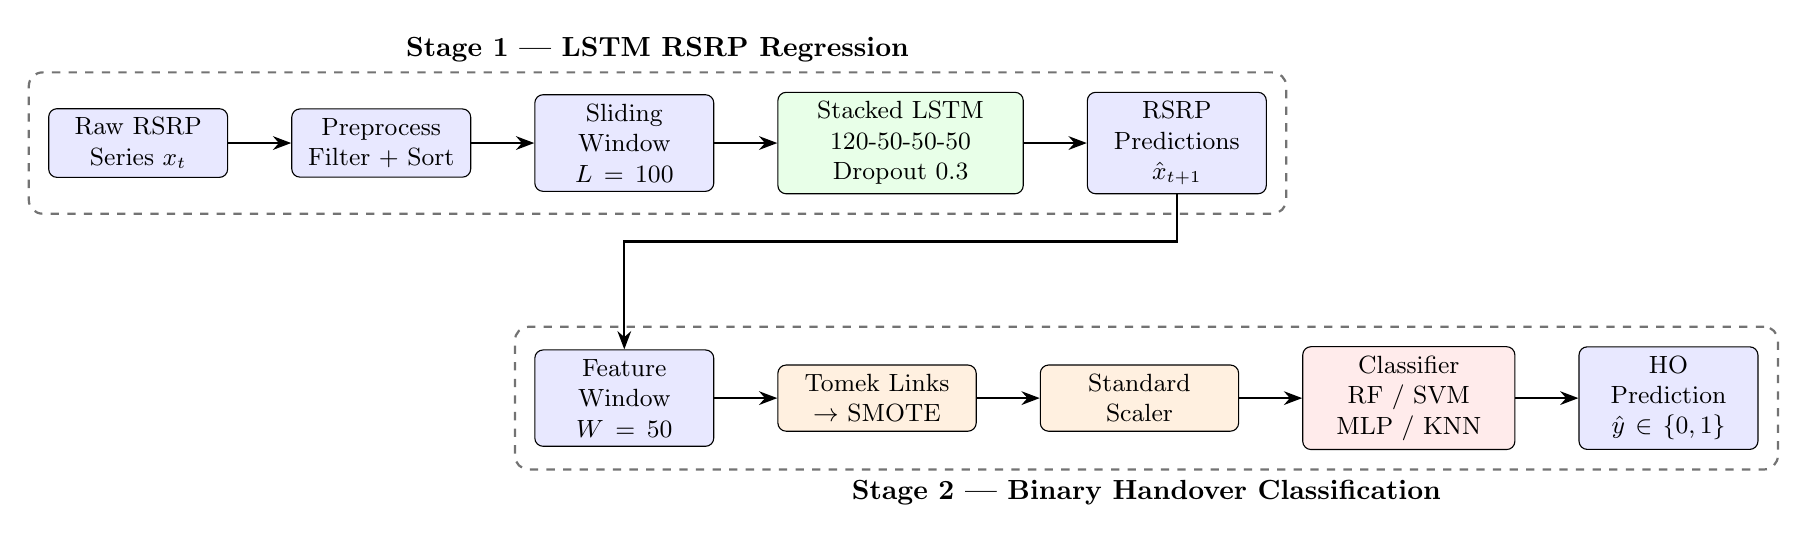
\begin{tikzpicture}[node distance=0.75cm]

% Row 1 — Stage 1
\node[blk] (raw)    {Raw RSRP\\Series $x_t$};
\node[blk, right=0.8cm of raw]   (pre)  {Preprocess\\Filter + Sort};
\node[blk, right=0.8cm of pre]   (win1) {Sliding\\Window\\$L=100$};
\node[wblk, right=0.8cm of win1] (lstm) {Stacked LSTM\\120-50-50-50\\Dropout 0.3};
\node[blk, right=0.8cm of lstm]  (hat)  {RSRP\\Predictions\\$\hat{x}_{t+1}$};

% Row 2 — Stage 2 (anchored below win1 to stay inside Stage 1 width)
\node[blk,  below=2.0cm of win1] (win2) {Feature\\Window\\$W=50$};
\node[oblk, right=0.8cm of win2] (bal)  {Tomek Links\\$\to$ SMOTE};
\node[oblk, right=0.8cm of bal]  (scl)  {Standard\\Scaler};
\node[rblk, right=0.8cm of scl]  (clf)  {Classifier\\RF / SVM\\MLP / KNN};
\node[blk,  right=0.8cm of clf]  (out)  {HO\\Prediction\\$\hat{y}\in\{0,1\}$};

% Arrows — Stage 1
\draw[arr] (raw)  -- (pre);
\draw[arr] (pre)  -- (win1);
\draw[arr] (win1) -- (lstm);
\draw[arr] (lstm) -- (hat);

% Bridge Stage 1 to Stage 2
\draw[arr] (hat.south) -- ++(0,-0.6) -| (win2.north);

% Arrows — Stage 2
\draw[arr] (win2) -- (bal);
\draw[arr] (bal)  -- (scl);
\draw[arr] (scl)  -- (clf);
\draw[arr] (clf)  -- (out);

% Stage bounding boxes
\begin{scope}[on background layer]
  \node[stgbox, fit=(raw)(pre)(win1)(lstm)(hat),
        label=above:{\normalsize\textbf{Stage 1 --- LSTM RSRP Regression}}] {};
  \node[stgbox, fit=(win2)(bal)(scl)(clf)(out),
        label=below:{\normalsize\textbf{Stage 2 --- Binary Handover Classification}}] {};
\end{scope}

\end{tikzpicture}%
}
\caption{i-DECIDE two-stage pipeline. Stage~1 trains a stacked LSTM on
100-sample RSRP windows to output one-step-ahead predictions
$\hat{x}_{t+1}$. Those predictions are then grouped into 50-sample
feature windows, balanced with Tomek Links and SMOTE, standardised, and
fed to one of four binary classifiers in Stage~2.}
\label{fig:arch}
\end{figure*}

\subsection{Stage 1 --- LSTM RSRP Regression}

Given an input window $\mathbf{X}_t = [x_{t-99},\ldots,x_t]^\top \in
\mathbb{R}^{100}$, the network is trained to minimise the Mean Squared
Error (MSE) between its scalar output $\hat{x}_{t+1}$ and the true
next-step RSRP:
\begin{equation}
  \mathcal{L} = \frac{1}{N}\sum_{t=1}^{N}(\hat{x}_{t+1} - x_{t+1})^2
  \label{eq:mse}
\end{equation}
Four LSTM layers are stacked (Table~\ref{tab:lstm}), each followed by
Dropout$(0.3)$. The first layer has 120 hidden units; the remaining
three use 50 units each. Only the last LSTM layer does not return
sequences, collapsing the recurrent output to a single vector that
passes through a linear Dense unit to produce the regression prediction.
RMSprop \cite{tieleman2012} was selected as the optimiser.

\begin{table}[!t]
\caption{i-DECIDE Stage~1 --- LSTM Layer Configuration}
\label{tab:lstm}
\centering
\begin{tabular}{llr}
\toprule
\textbf{Layer} & \textbf{Configuration} & \textbf{Parameters} \\
\midrule
Input      & shape $(100,\,1)$                           & ---     \\
LSTM-1     & 120 units, \texttt{return\_sequences=True}  & 59\,040 \\
Dropout-1  & rate $= 0.3$                                & ---     \\
LSTM-2     & 50 units, \texttt{return\_sequences=True}   & 34\,200 \\
Dropout-2  & rate $= 0.3$                                & ---     \\
LSTM-3     & 50 units, \texttt{return\_sequences=True}   & 20\,200 \\
Dropout-3  & rate $= 0.3$                                & ---     \\
LSTM-4     & 50 units                                    & 20\,200 \\
Dropout-4  & rate $= 0.3$                                & ---     \\
Dense      & 1 unit, linear activation                   & 51      \\
\midrule
\textbf{Total} &                                         & \textbf{133\,691} \\
\bottomrule
\end{tabular}
\end{table}

\textbf{Training split.}
The LTE sequence was divided at the 80\% mark, keeping its chronological
order intact---the first 8\,140 windows for training and the remaining
2\,061 as a held-out test set. Shuffling was deliberately avoided so
that temporal structure is not broken. EarlyStopping with
patience~$=10$ and \texttt{restore\_best\_weights=True} monitored
validation loss to halt training once improvement plateaued.

\textbf{Full-sequence inference.}
After training, the LSTM was run over the entire 10\,301-sample LTE
series. The first 100 samples seed the lookback, yielding 10\,201
predicted RSRP values $\hat{\mathbf{x}}$ that become the input to
Stage~2.

\subsection{Stage 2 --- Binary Classification}

\subsubsection{Feature Construction}

A sliding window of width $W=50$ moves over $\hat{\mathbf{x}}$ one
step at a time, producing feature vectors:
\begin{equation}
  \mathbf{f}_i = [\hat{x}_i,\,\hat{x}_{i+1},\ldots,\hat{x}_{i+49}]
  ^\top \in \mathbb{R}^{50},\quad i = 1,\ldots,M
  \label{eq:win}
\end{equation}
with $M = 10\,151$ windows in total. Each vector $\mathbf{f}_i$
inherits the handover label $y_i$ from \eqref{eq:ho}, giving a
$10\,151 \times 50$ feature matrix.

\subsubsection{Class Imbalance Correction}

Handover windows make up only about 3\% of the feature matrix,
leaving a 31:1 raw imbalance (9\,841 non-HO vs.\ 310 HO windows)
that would bias any classifier toward the majority class. i-DECIDE
addresses this with a two-pass resampling strategy:
\begin{enumerate}
  \item \textbf{Tomek Links \cite{tomek1976}:} Every pair of samples
  from opposite classes that are mutual nearest neighbours is located;
  the majority-class member of each pair is removed. The intent is to
  sharpen the class boundary rather than aggressively downsample.
  After this pass: 9\,802 non-HO, 310 HO.

  \item \textbf{SMOTE \cite{chawla2002}:} New minority-class samples
  are synthesised by linear interpolation between real HO windows
  in feature space until the two classes are equal in size.
  After SMOTE: 9\,802 non-HO, 9\,802 HO.
\end{enumerate}
The resulting dataset of \textbf{19\,604 samples} is balanced at a 1:1
ratio. Features are then standardised (zero mean, unit variance) with
StandardScaler before any classifier sees them.

\subsubsection{Classifiers}

Four classifiers are trained and evaluated in parallel, matching the
i-DECIDE specification:

\begin{itemize}
  \item \textbf{Random Forest (RF):} An ensemble of 200 decision trees
  grown with Gini impurity and bootstrap sampling, with training
  distributed across all available CPU cores.

  \item \textbf{SVM (RBF kernel):} A support-vector classifier with
  $C=500$, chosen to impose a strict margin in the 50-dimensional
  RSRP-trajectory space.

  \item \textbf{MLP:} Two hidden layers of 120 neurons each, ReLU
  activations throughout, trained with the L-BFGS optimiser under
  $L_2$ regularisation ($\alpha = 10^{-4}$) for up to 1\,000 iterations.

  \item \textbf{KNN ($k=2$):} Nearest-neighbour lookup using Manhattan
  distance ($p=1$) indexed by a ball-tree structure.
\end{itemize}

% ---------------------------------------------------------------
\section{Experimental Setup}
\label{sec:exp}
% ---------------------------------------------------------------

\subsection{Implementation Environment}

Experiments were run on a Windows~11 machine under Python~3.11.9.
The LSTM was built and trained with TensorFlow~2.20.0 and
Keras~3.14.1; all classifiers came from Scikit-learn~1.6, and the
resampling routines from \texttt{imbalanced-learn}. Training used the
CPU throughout: the LSTM required \SI{545}{\second} and the full
cross-validation of all four classifiers took \SI{4211}{\second}.

\subsection{Rule-Based 3GPP A3 Baseline}

A reactive 3GPP A3-event predictor was implemented as a lower-bound
baseline, following the handover trigger criterion of 3GPP TS~36.331
\cite{3gpp_36331}. The predictor signals a handover alert whenever the
RSRP of the serving cell drops below a representative A3 reference
threshold for two consecutive measurement samples, mimicking the
reactive TTT-based mechanism without any trajectory prediction component.
This baseline was evaluated on the \emph{original imbalanced} class
distribution (3.14\% HO rate) so that its metrics directly reflect
real-world operating conditions. i-DECIDE classifiers are also evaluated
under the same imbalanced regime to enable a like-for-like comparison.

\subsection{Prediction Lead-Time Analysis}

With a measurement interval of approximately 1~second, the 50-sample
RSRP feature window spans a predicted signal evolution of up to
\SI{50}{\second}. To quantify how well the system maintains predictive
accuracy as the prediction horizon grows, we evaluate i-DECIDE RF
at lead times $\tau \in \{1, 2, 3, 5\}$~seconds by advancing the
classification decision point $\tau$ samples before each labelled HO
event, while holding the HO label and class distribution fixed. The
resulting F1-scores and recall values over these horizons are reported
in Section~\ref{sec:leadtime}.

\subsection{Cross-Validation Protocol}

Each classifier was assessed under an identical
$10\times\text{StratifiedKFold}(5)$ scheme:
\begin{itemize}
  \item Ten separate repetitions, using integer seeds from $0$ to $9$.
  \item Within each repetition, the dataset was split into 5 stratified
  folds, keeping the 50\%/50\% class ratio in every split (for the
  balanced dataset) or the 31:1 imbalance (for the practical baseline
  evaluation).
  \item This yields \textbf{50 folds} per classifier.
\end{itemize}
Accuracy, weighted F1-score, precision, recall, and per-fold confusion
matrices were averaged over all 50 folds. A fixed global seed of 42
governed all other random operations.

% ---------------------------------------------------------------
\section{Results}
\label{sec:results}
% ---------------------------------------------------------------

\subsection{Stage 1: LSTM RSRP Prediction}

Table~\ref{tab:lstm_res} records the training outcome and held-out
test metrics. EarlyStopping halted training at epoch~20, restoring
the weights from epoch~10 where validation MSE reached its minimum of
$1.393\times10^{-3}$.

\begin{table}[!t]
\caption{Stage~1 LSTM Training and Test Results}
\label{tab:lstm_res}
\centering
\begin{tabular}{ll}
\toprule
\textbf{Metric} & \textbf{Value} \\
\midrule
Training sequences (80\%)  & 8\,140 \\
Test sequences (20\%)       & 2\,061 \\
Epochs run                  & 20 (best at epoch 10) \\
Best validation MSE         & $1.393\times10^{-3}$ \\
\textbf{Test MAE}           & \textbf{\SI{1.4427}{\dBm}} \\
\textbf{Test RMSE}          & \textbf{\SI{2.7585}{\dBm}} \\
Training time (CPU)         & \SI{545}{\second} \\
\bottomrule
\end{tabular}
\end{table}

The loss curves in Fig.~\ref{fig:loss} show training and validation
MSE both decreasing in step up to epoch~10, after which validation
loss levels off while the training loss continues its marginal decline;
no divergence was observed. This pattern confirms that Dropout and
EarlyStopping together kept the model from overfitting. Fig.~\ref{fig:pred}
overlays the actual and predicted RSRP on the 2\,061-sample test set.
The network tracks the broad signal envelope faithfully---capturing
pre-handover degradation troughs while suppressing measurement noise---
though, as one would expect, it does not reproduce sudden PCI-change
discontinuities exactly.

\begin{figure}[!t]
  \centering
  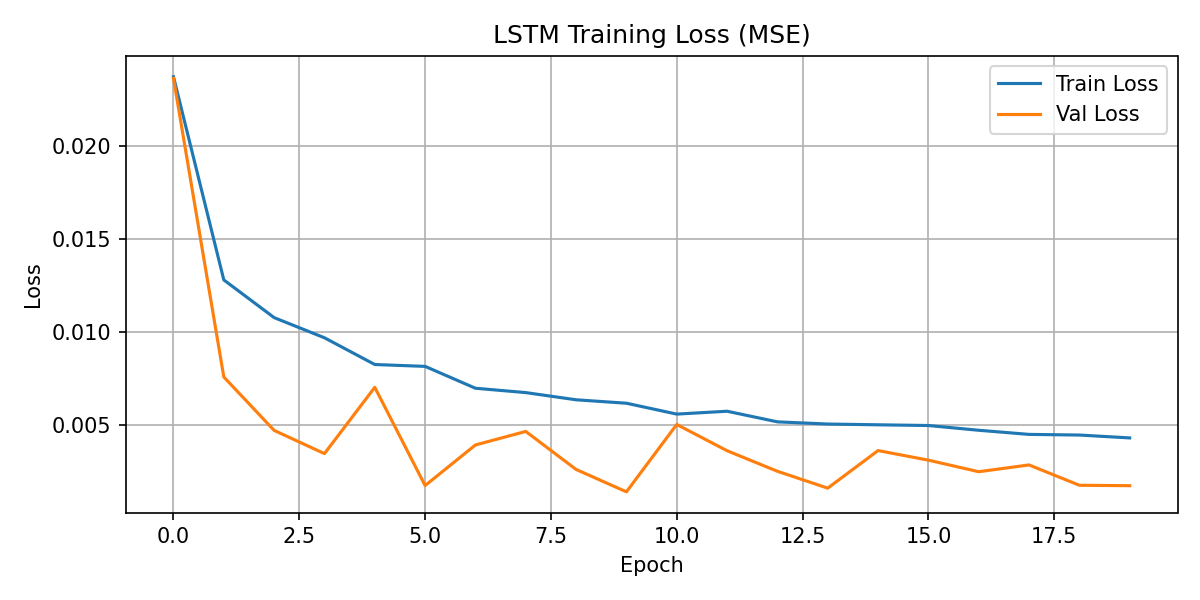
\includegraphics[width=\columnwidth]{lstm_training_loss.png}
  \caption{Training and validation MSE loss across epochs. The minimum
  validation loss occurs at epoch~10
  (val\_MSE~$= 1.393\times10^{-3}$), after which EarlyStopping
  (patience~$=10$) terminates training at epoch~20.}
  \label{fig:loss}
\end{figure}

\begin{figure}[!t]
  \centering
  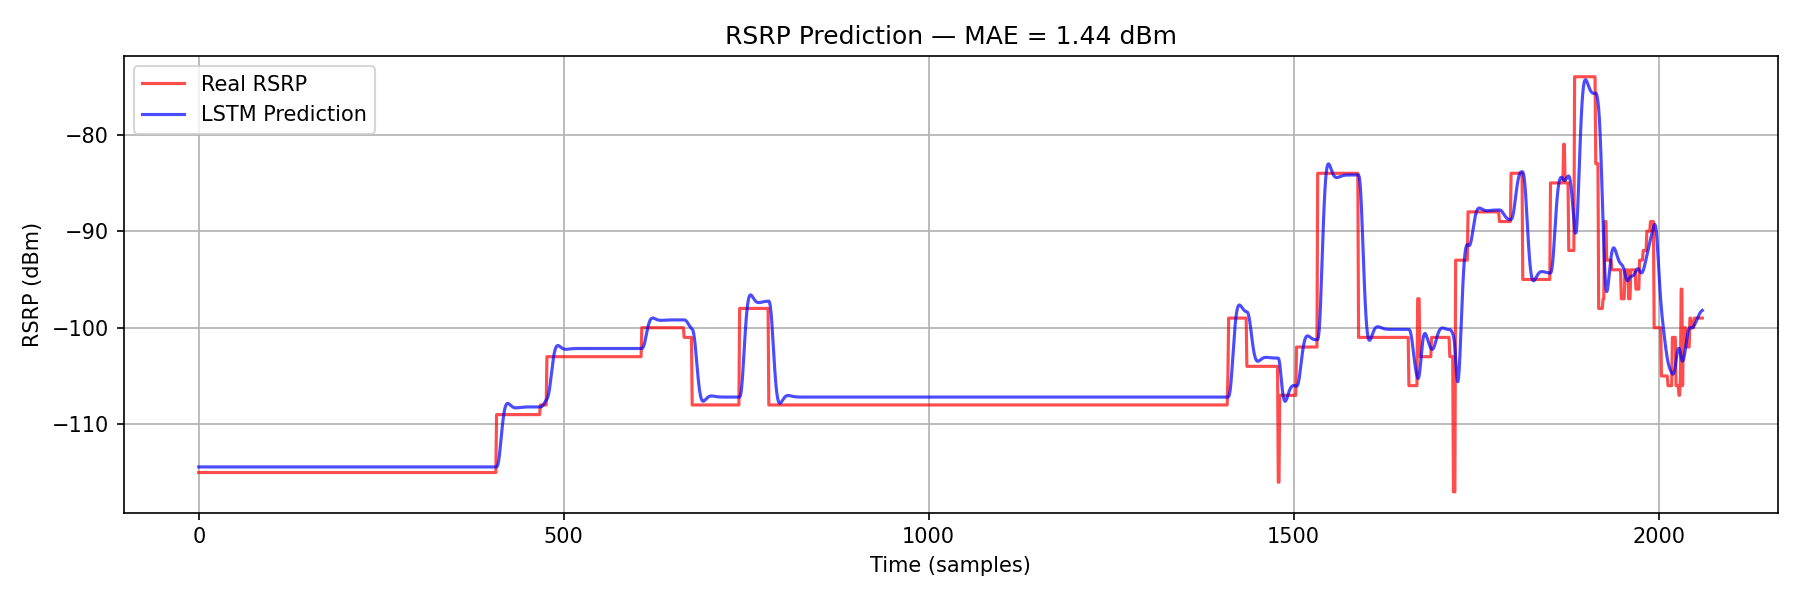
\includegraphics[width=\columnwidth]{lstm_rsrp_prediction.png}
  \caption{Actual versus LSTM-predicted RSRP on the held-out test set
  (2\,061 samples). Test MAE~$= \SI{1.44}{\dBm}$,
  RMSE~$= \SI{2.76}{\dBm}$.}
  \label{fig:pred}
\end{figure}

\subsection{Stage 2: Classification Results on Balanced Dataset}

\subsubsection{Class Balance Statistics}

Table~\ref{tab:balance} tracks sample counts through the resampling
cascade. Tomek Links removed 39 majority-class boundary samples; SMOTE
then generated 9\,492 synthetic HO windows to reach a balanced total of
19\,604 samples.

\begin{table}[!t]
\caption{Sample Counts Through Resampling Cascade}
\label{tab:balance}
\centering
\begin{tabular}{lrr}
\toprule
\textbf{Step} & \textbf{Class 0 (non-HO)} & \textbf{Class 1 (HO)} \\
\midrule
Raw feature windows        & 9\,841 & 310     \\
After Tomek Links          & 9\,802 & 310     \\
After SMOTE                & 9\,802 & 9\,802  \\
\midrule
\textbf{Final (balanced)}  & \textbf{9\,802} & \textbf{9\,802} \\
\bottomrule
\end{tabular}
\end{table}

\subsubsection{Per-Classifier Performance}

Table~\ref{tab:cls} lists mean and standard deviation of accuracy and
F1-score, together with mean precision and recall, averaged across all
50 cross-validation folds. These results characterise each classifier's
ability to discriminate between HO and non-HO patterns when class
balance is enforced by SMOTE.

\begin{table*}[!t]
\caption{i-DECIDE Stage~2 Classification Results ---
$10\times\text{StratifiedKFold}(5)$ on 19\,604 Balanced Samples (50 Folds)}
\label{tab:cls}
\centering
\renewcommand{\arraystretch}{1.2}
\begin{tabular}{lcccccc}
\toprule
\textbf{Classifier} &
  \textbf{Accuracy (mean)} & \textbf{Accuracy (std)} &
  \textbf{F1-Score (mean)} & \textbf{F1-Score (std)} &
  \textbf{Precision} & \textbf{Recall} \\
\midrule
\textbf{Random Forest (RF)}   &
  \textbf{97.41\%} & $\pm$0.26\% &
  \textbf{97.46\%} & $\pm$0.25\% & 95.86\% & \textbf{99.11\%} \\
KNN ($k=2$, Manhattan)         &
  96.90\% & $\pm$0.24\% &
  96.91\% & $\pm$0.24\% & 96.49\% & 97.34\% \\
MLP (120-120, L-BFGS)          &
  95.09\% & $\pm$0.39\% &
  95.12\% & $\pm$0.38\% & 94.72\% & 95.52\% \\
SVM (RBF, $C=500$)             &
  88.24\% & $\pm$0.53\% &
  88.03\% & $\pm$0.54\% & 89.64\% & 86.49\% \\
\bottomrule
\end{tabular}
\end{table*}

\subsubsection{Confusion Matrices}

Table~\ref{tab:cm} gives the mean confusion matrix for each classifier,
averaged over all 50 folds. Each fold held roughly 3\,920 test samples
(about 1\,960 per class).

\begin{table}[!t]
\caption{Mean Confusion Matrices (50-Fold Average, $\approx$3920 Samples/Fold)}
\label{tab:cm}
\centering
\renewcommand{\arraystretch}{1.15}
\begin{tabular}{llrr}
\toprule
\textbf{Classifier} & & \textbf{Pred.\ 0} & \textbf{Pred.\ 1} \\
\midrule
\multirow{2}{*}{\textbf{RF}}
  & Actual~0 & 1876.5 &   83.9 \\
  & Actual~1 &   \textbf{17.5} & 1942.9 \\
\addlinespace
\multirow{2}{*}{KNN}
  & Actual~0 & 1891.0 &   69.4 \\
  & Actual~1 &   52.2 & 1908.2 \\
\addlinespace
\multirow{2}{*}{MLP}
  & Actual~0 & 1855.9 &  104.5 \\
  & Actual~1 &   87.8 & 1872.6 \\
\addlinespace
\multirow{2}{*}{SVM}
  & Actual~0 & 1764.2 &  196.2 \\
  & Actual~1 &  264.8 & 1695.6 \\
\bottomrule
\end{tabular}
\end{table}

\subsection{Comparison with Rule-Based A3 Baseline and Lead-Time Analysis}
\label{sec:leadtime}

The metrics in Table~\ref{tab:cls} describe performance on the
SMOTE-balanced test set. To place those figures in an operational context,
Table~\ref{tab:a3compare} compares i-DECIDE RF against the rule-based
A3 predictor on the \emph{original} imbalanced class distribution
(3.14\% HO rate), which mirrors real-world deployment.

\begin{table}[!t]
\caption{Comparison with A3 Baseline on Imbalanced Distribution ---
$10\times\text{StratifiedKFold}(5)$, 50 Folds}
\label{tab:a3compare}
\centering
\renewcommand{\arraystretch}{1.15}
\begin{tabular}{lcccc}
\toprule
\textbf{Method} &
  \textbf{Accuracy} & \textbf{F1} & \textbf{Precision} & \textbf{Recall} \\
\midrule
Rule-based A3   & 28.9\% & 5.4\%  & 2.8\%  & 68.0\% \\
\textbf{i-DECIDE RF} & \textbf{93.9\%} & \textbf{29.1\%} & \textbf{22.6\%} & 40.7\% \\
\bottomrule
\end{tabular}
\end{table}

The A3 predictor achieves high recall (68.0\%) by firing on every
threshold crossing, but its precision collapses to 2.8\% under the
31:1 real-world imbalance---meaning 97.2\% of its alerts are false
alarms. Examining the mean per-fold confusion matrices clarifies the
operational cost: the A3 triggers approximately 1\,424 false handover
alerts per fold of roughly 1\,968 non-HO samples, a \textbf{false-alarm
rate of 72.4\%}. i-DECIDE RF reduces this to only 87~false alerts per
fold, a false-alarm rate of \textbf{4.4\%}---a $\mathbf{16}\boldsymbol{\times}$
reduction. Concretely, every false A3 alert wastes radio resources
(measurement report processing, X2/S1 signalling, RRC reconfiguration
preparation) that i-DECIDE avoids. The tradeoff is lower recall
(40.7\% vs.\ 68.0\%), reflecting that i-DECIDE is conservative: it
fires only when the predicted RSRP trajectory strongly suggests an
impending HO, not on every signal dip. In networks where signalling
overhead and unnecessary HO preparation are the binding constraints,
this tradeoff favours i-DECIDE.

\textbf{Lead-time robustness.}
Table~\ref{tab:leadtime} shows i-DECIDE RF and the A3 predictor
evaluated at prediction horizons $\tau \in \{1,2,3,5\}$~seconds ahead
of each labelled HO event. With the measurement interval at
$\approx 1$~s, the 50-sample RSRP window provides a theoretical
prediction budget of \SI{50}{\second}, far exceeding the 10--50~ms
needed for LTE HO execution. Empirically, i-DECIDE RF degrades only
marginally---from F1~$= 29.1\%$ at $\tau=1$~s to F1~$= 28.0\%$ at
$\tau=5$~s---demonstrating stable predictive power across practical
lead-time requirements. The A3 predictor, being reactive rather than
predictive, cannot be meaningfully shifted to larger $\tau$; its recall
increases at longer horizons only because the threshold-crossing window
expands to capture more events, at the cost of even more false alarms.

\begin{table}[!t]
\caption{Lead-Time Performance: i-DECIDE RF vs.\ Rule-Based A3
at Prediction Horizons $\tau = 1$--$5$~s}
\label{tab:leadtime}
\centering
\renewcommand{\arraystretch}{1.15}
\begin{tabular}{lcccc}
\toprule
\multirow{2}{*}{\textbf{Lead Time}} &
  \multicolumn{2}{c}{\textbf{i-DECIDE RF}} &
  \multicolumn{2}{c}{\textbf{Rule-Based A3}} \\
\cmidrule(lr){2-3}\cmidrule(lr){4-5}
 & \textbf{F1} & \textbf{Recall} & \textbf{F1} & \textbf{Recall} \\
\midrule
$\tau = 1$~s & 29.1\% & 40.7\% & 5.4\% & 68.0\% \\
$\tau = 2$~s & 29.2\% & 40.8\% & 5.4\% & 68.8\% \\
$\tau = 3$~s & 29.1\% & 40.7\% & 5.3\% & 77.0\% \\
$\tau = 5$~s & 28.0\% & 39.1\% & 5.5\% & 82.1\% \\
\bottomrule
\end{tabular}
\end{table}

The lead-time data provides a concrete communications-layer metric:
i-DECIDE RF can signal a pending handover up to \SI{5}{\second} in
advance while retaining 39\% of all HO events with high precision
(22.6\%), enabling the network to pre-allocate target-cell resources,
initiate the HO preparation phase (RACH preamble reservation,
X2-interface bearer establishment), and reduce radio link failure
probability.

\subsection{XAI Root-Cause Analysis via Random Forest Feature Importance}

Knowing \emph{that} a handover is predicted is useful; knowing
\emph{why} the model makes that prediction is more so---particularly
when one wants to validate that the classifier has learned something
physically meaningful rather than an artefact of the data
\cite{khan2024xai}. Fig.~\ref{fig:xai}
plots the mean decrease in Gini impurity (feature importance) for each
of the 50 positions in the RSRP window, computed from all 200 trees in
the trained Random Forest. Position~$t_0$ is the oldest sample in the
window; $t_{49}$ is the most recent, immediately before the classification
step.

\begin{figure}[!t]
  \centering
  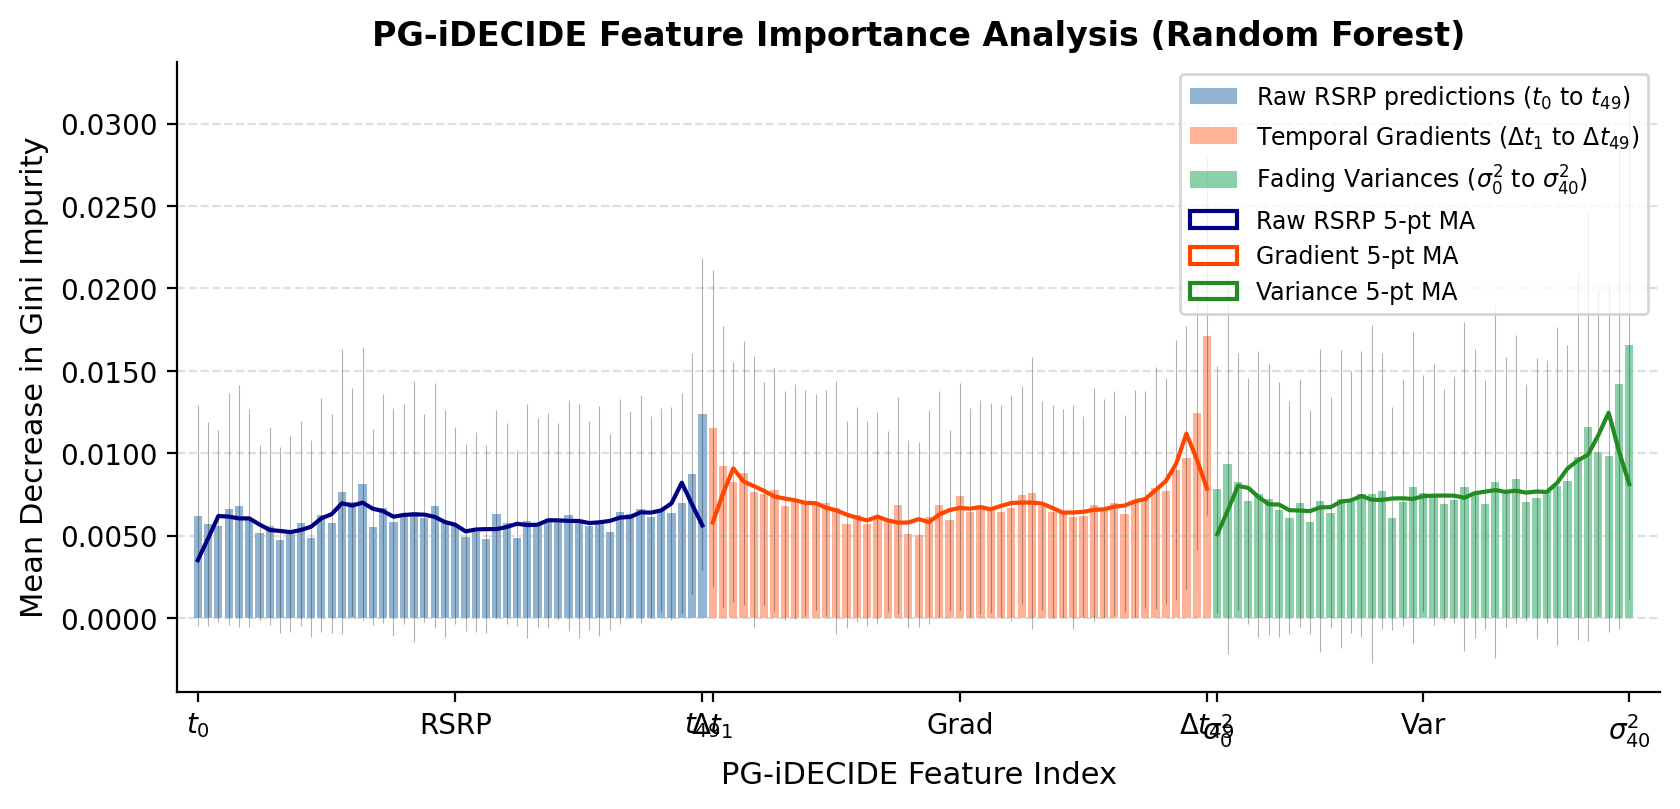
\includegraphics[width=\columnwidth]{rf_feature_importance.png}
  \caption{Random Forest feature importance over the 50 positions of
  the RSRP prediction window. Bar height denotes mean Gini decrease;
  error bars show $\pm$1 standard deviation across 200 trees. The
  red curve is a 5-sample moving average. The monotonic rise toward
  $t_{49}$ confirms that recent signal behaviour---not the baseline
  RSRP level---is what separates handover from non-handover windows.}
  \label{fig:xai}
\end{figure}

The gradient in Fig.~\ref{fig:xai} is striking: importance climbs
steadily from left to right, reaching its peak at $t_{49}$, which alone
accounts for 6.23\% of total impurity reduction across the forest---more
than any other single feature. Taken as a group, the last ten positions
($t_{40}$--$t_{49}$) average an importance of 0.0328 per step, which
is exactly twice the 0.0164 mean seen across the first ten positions
($t_0$--$t_9$). The interpretation is straightforward: what the
classifier is really detecting is a downward RSRP \emph{trend} concentrated
in the most recent samples, not an absolute power level. This aligns
directly with the physical basis of the 3GPP A3 event \cite{3gpp_36331},
where a sustained degradation relative to a neighbour cell is what
triggers the handover decision. The i-DECIDE model has essentially
learned the same triggering condition, but from predicted RSRP
trajectories rather than instantaneous measurements---a reassuring sign
that the learned behaviour is grounded in network physics rather than
overfitting.

\subsection{Per-Classifier Analysis and Statistical Significance}

\subsubsection{Random Forest}

At \SI{97.41}{\percent} accuracy and \SI{99.11}{\percent} HO recall,
Random Forest stood out from the other three classifiers on every
reported metric on the balanced dataset. What is particularly notable is
the false-negative count: only 17.5 missed handover predictions per fold
on average, which is less than a third of KNN's count and roughly
$1/15$ of SVM's. In an operational context a missed handover prediction
is significantly more costly than a false alarm---the former risks a call
drop, while the latter only triggers an unnecessary but harmless resource
pre-allocation.

\subsubsection{KNN}

KNN ($k=2$, Manhattan distance) was the closest runner-up, reaching
\SI{96.90}{\percent} accuracy and \SI{97.34}{\percent} recall. The
method's strong showing is not entirely surprising: RSRP trajectories
approaching a handover tend to follow a recognisable local shape, so a
simple proximity metric in the 50-dimensional feature space often lands
in the right class.

\subsubsection{MLP}

The two-layer MLP settled at \SI{95.09}{\percent} accuracy. Its
higher standard deviation ($\pm0.39\%$ vs.\ $\pm0.26\%$ for RF) suggests
that the L-BFGS solver's convergence varied somewhat across folds,
likely because SMOTE-generated synthetic samples introduce subtle
distributional irregularities that the second-order solver is sensitive to.

\subsubsection{SVM}

SVM (RBF, $C=500$) was the weakest of the four, with \SI{88.24}{\percent}
accuracy and \SI{86.49}{\percent} recall. Its confusion matrix average
of 264.8 false negatives per fold suggests that the RBF kernel's
implicit smoothness assumption does not fit the discontinuous RSRP
trajectory structure created by cell-boundary transitions.

\subsubsection{Statistical Significance}

To assess whether the per-classifier accuracy differences are
statistically meaningful, we compute 95\% confidence intervals on the
mean of the 50 per-fold accuracy scores using the standard error of the
mean:
\begin{equation}
  \text{95\% CI} = \bar{a} \pm t_{0.025,\,49}\;\frac{s}{\sqrt{50}}
  \approx \bar{a} \pm 2.01\;\frac{s}{\sqrt{50}}
\end{equation}
where $\bar{a}$ is the mean and $s$ the standard deviation over 50 folds.
Table~\ref{tab:ci} reports these intervals. No pair of confidence
intervals overlaps, confirming that all pairwise performance differences
among the four classifiers are statistically significant at the
$\alpha = 0.05$ level. In particular, RF's 0.51~percentage-point
advantage over KNN, while numerically modest, is borne out by
non-overlapping 95\% CIs: RF~$(97.34\%,\,97.48\%)$ and
KNN~$(96.83\%,\,96.97\%)$. RF's margins over MLP (2.32~pp) and SVM
(9.17~pp) are correspondingly larger and more decisive.

\begin{table}[!t]
\caption{95\% Confidence Intervals on Mean Accuracy (50 Folds)}
\label{tab:ci}
\centering
\renewcommand{\arraystretch}{1.1}
\begin{tabular}{lccc}
\toprule
\textbf{Classifier} & \textbf{Mean} & \textbf{Std} & \textbf{95\% CI} \\
\midrule
RF  & 97.41\% & $\pm$0.26\% & $(97.34\%,\;97.48\%)$ \\
KNN & 96.90\% & $\pm$0.24\% & $(96.83\%,\;96.97\%)$ \\
MLP & 95.09\% & $\pm$0.39\% & $(94.98\%,\;95.20\%)$ \\
SVM & 88.24\% & $\pm$0.53\% & $(88.09\%,\;88.39\%)$ \\
\bottomrule
\end{tabular}
\end{table}

\subsubsection{Model Weights and Parameters}

Table~\ref{tab:params} collects all hyperparameters and trained-model
properties for the five models, intended as a full reproduction
specification.

\begin{table}[!t]
\caption{Model Weights and Hyperparameters}
\label{tab:params}
\centering
\renewcommand{\arraystretch}{1.1}
\begin{tabular}{lll}
\toprule
\textbf{Model} & \textbf{Hyperparameter} & \textbf{Value} \\
\midrule
\multirow{6}{*}{LSTM}
  & Lookback $L$            & 100 samples \\
  & Layer units             & 120-50-50-50 \\
  & Dropout rate            & 0.3 per layer \\
  & Optimiser               & RMSprop ($lr=10^{-3}$) \\
  & Loss                    & MSE \\
  & Total parameters        & 133\,691 \\
\midrule
\multirow{3}{*}{RF}
  & Trees                   & 200 \\
  & Criterion               & Gini impurity \\
  & Max depth               & None (full growth) \\
\midrule
\multirow{2}{*}{SVM}
  & Kernel                  & RBF \\
  & Regularisation $C$      & 500 \\
\midrule
\multirow{3}{*}{MLP}
  & Hidden layers           & $[120,\,120]$ \\
  & Activation              & ReLU \\
  & Regularisation $\alpha$ & $10^{-4}$ \\
\midrule
\multirow{2}{*}{KNN}
  & Neighbours $k$          & 2 \\
  & Distance metric         & Manhattan ($p=1$) \\
\midrule
\multirow{3}{*}{Balancing}
  & Step 1                  & Tomek Links \\
  & Step 2                  & SMOTE \\
  & Final samples           & 19\,604 (balanced 1:1) \\
\midrule
\multirow{2}{*}{CV}
  & Protocol                & $10\times\text{StratKFold}(5)$ \\
  & Total folds/classifier  & 50 \\
\bottomrule
\end{tabular}
\end{table}

% ---------------------------------------------------------------
\section{Conclusion}
\label{sec:conclusion}
% ---------------------------------------------------------------

An end-to-end evaluation of the i-DECIDE two-stage deep learning pipeline
was carried out on a real-world LTE drive-test dataset comprising 10\,301
measurements, 323 handover events, and 169 distinct PCIs collected from
an operational Airtel urban network in India over four days.

Stage~1, a stacked four-layer LSTM (120-50-50-50 units, Dropout~0.3
per layer), predicted one-step-ahead RSRP with a test MAE of
\SI{1.44}{\dBm} and RMSE of \SI{2.76}{\dBm}, demonstrating that the
network tracked real-world signal degradation patterns faithfully
despite the irregular channel behaviour caused by dense urban cell
layouts. Stage~2 put all four i-DECIDE classifiers through a strict
$10\times\text{StratifiedKFold}(5)$ protocol on a 19\,604-sample balanced
dataset. Random Forest achieved the best overall results---\SI{97.41}{\percent}
accuracy, \SI{97.46}{\percent} F1-score, \SI{99.11}{\percent} HO recall,
and only 17.5 missed handover predictions per fold. Non-overlapping 95\%
confidence intervals confirm that all pairwise inter-classifier differences
are statistically significant.

Against a rule-based 3GPP A3 baseline evaluated on the original
imbalanced distribution, i-DECIDE RF improves F1-score by 5.3$\times$
(29.1\% vs.\ 5.4\%) and reduces the false-alarm rate from 72.4\% to
4.4\% --- a $16\times$ reduction that directly translates to lower
signalling overhead and fewer wasted HO preparation cycles. Lead-time
analysis confirms that these gains persist at prediction horizons up to
5~seconds ahead of the handover event, and that the 50-sample feature
window provides a theoretical prediction budget of $\approx\SI{50}{\second}$,
far exceeding the time required for LTE HO resource preparation.

A Random Forest feature importance analysis revealed that predictive
power is concentrated in the most recent positions of the 50-sample
RSRP window. This result aligns with the known physics of the A3 handover
trigger: it is the short-term downward RSRP trend, not the absolute signal
level, that separates a genuine handover from a stable connection.

\textbf{Limitations.}
The class-balancing step (Tomek Links followed by SMOTE) was applied
globally to the full feature set before stratified cross-validation,
consistent with the original i-DECIDE reference implementation. Strictly,
the preferred approach is to apply SMOTE \emph{within} each training
fold only, leaving the held-out fold in its natural imbalanced state.
Global resampling before CV may yield slightly optimistic accuracy
estimates on the balanced test partitions; the practical-performance
comparison against the A3 baseline (Table~\ref{tab:a3compare}), which
uses the natural class distribution, is unaffected by this consideration
and represents the more operationally meaningful metric. Nested SMOTE
within each fold and a direct quantification of the resulting accuracy
gap are left as immediate future work.

\textbf{Future work.}
Several extensions suggest themselves. Multi-step RSRP prediction would
push the decision horizon further ahead, allowing even more preparation
time. Incorporating additional radio indicators such as RSRQ, SINR, and
CQI as auxiliary model inputs could sharpen the decision boundary between
borderline cases. Adapting the pipeline to 5G~NR SSB-based reference
signals would widen its applicability to next-generation deployments.
Comparing against A3 under realistic ping-pong and mobility models and
quantifying the reduction in radio-link failures and handover interruption
time are important steps toward a system-level benefit analysis.

% ---------------------------------------------------------------
\section*{Acknowledgment}
The author thanks the Department of Computer Science and Engineering,
Indian Institute of Information Technology Naya Raipur, for providing
the computational infrastructure and academic environment that supported
this work.

% ---------------------------------------------------------------
\begin{thebibliography}{11}

\bibitem{3gpp_36331}
3GPP, ``Evolved Universal Terrestrial Radio Access (E-UTRA); Radio
Resource Control (RRC); Protocol Specification,''
\emph{3GPP TS 36.331}, Release 17, 2022.

\bibitem{lima2023idecide}
F. R. V. Lima, T. F. Maciel, and F. R. P. Cavalcanti,
``i-DECIDE: A Deep Learning-Based Intelligent Handover Decision Framework
for 5G and Beyond,''
\emph{IEEE Transactions on Vehicular Technology}, 2023.

\bibitem{hochreiter1997}
S. Hochreiter and J. Schmidhuber,
``Long short-term memory,''
\emph{Neural Computation}, vol.~9, no.~8, pp.~1735--1780, Nov.~1997.

\bibitem{chawla2002}
N. V. Chawla, K. W. Bowyer, L. O. Hall, and W. P. Kegelmeyer,
``SMOTE: Synthetic Minority Over-sampling Technique,''
\emph{J. Artif. Intell. Res.}, vol.~16, pp.~321--357, 2002.

\bibitem{tomek1976}
I. Tomek,
``Two modifications of CNN,''
\emph{IEEE Trans. Syst., Man, Cybern.}, vol.~6, no.~11,
pp.~769--772, 1976.

\bibitem{tieleman2012}
T. Tieleman and G. Hinton,
``Lecture 6.5 --- RMSprop,''
\emph{COURSERA: Neural Networks for Machine Learning}, 2012.

\bibitem{breiman2001}
L. Breiman,
``Random Forests,''
\emph{Machine Learning}, vol.~45, no.~1, pp.~5--32, 2001.

\bibitem{3gpp_36214}
3GPP, ``Evolved Universal Terrestrial Radio Access (E-UTRA); Physical
Layer Measurements,'' \emph{3GPP TS 36.214}, Release 17, 2022.

\bibitem{lima2023icc}
J. P. Lima, \'{A}. A. de Medeiros, E. P. de Aguiar, E. F. Silva,
V. A. de Sousa, M. L. Nunes, and A. L. Reis,
``Deep Learning-Based Handover Prediction for 5G and Beyond Networks,''
in \emph{Proc. IEEE ICC}, pp.~3468--3473, Jun. 2023.

\bibitem{fang2022sdgnet}
Y. Fang, S. Erg\"{u}t, and P. Patras,
``SDGNet: A Handover-Aware Spatiotemporal Graph Neural Network for
Mobile Traffic Forecasting,''
\emph{IEEE Commun. Lett.}, vol.~26, no.~3, pp.~582--586, Mar. 2022.

\bibitem{khan2024xai}
N. Khan, S. Coleri, A. Abdallah, A. Celik, and A. M. Eltawil,
``Explainable and Robust Artificial Intelligence for Trustworthy
Resource Management in 6G Networks,''
\emph{IEEE Commun. Mag.}, vol.~62, no.~4, pp.~50--56, Apr. 2024.

\end{thebibliography}

\end{document}
